\section{ALU}

Η μονάδα αριθμητικών και λογικών πράξεων (ALU) του σχήματος \ref{schematic:alu} έχει δύο εισόδους των 32 bit για τους τελεσταίους και μία είσοδο 4 bit για τον κωδικό της προς εκτέλεση πράξης. Το αποτέλεσμα της πράξης εμφανίζεται στην εξόδο των 32 bit. Τέλος, εάν το αποτέλεσμα της πράξης είναι μηδέν τότε ενεργοποιείται η έξοδος zero.\par

\begin{circuitfig}[H]
	\centering
	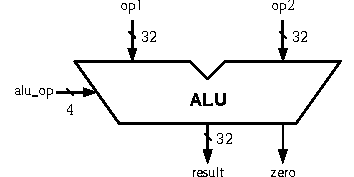
\includegraphics[width=6cm]{schematics/alu.pdf}
	\caption{Arithmetic logic unit (ALU). Οι είσοδοι των τελεσταίων είναι ακέραιοι αριθμοί.}
	\label{schematic:alu}
\end{circuitfig}

Οι πράξεις που υποστηρίζει η μονάδα είναι οι εξής:
\begin{enumerate}[itemsep=-0.5ex]
	\item πρόσθεση: $\text{op1}+\text{op2}$
	\item αφαίρεση: $\text{op1}-\text{op2}$
	\item αριθμητική ολίσθηση δεξιά: $\text{op1}\ggg\text{op2}[4:0]$
	\item λογική σύζευξη: $\text{op1}\land\text{op2}$
	\item λογική διάζευξη: $\text{op1}\lor\text{op2}$
	\item λογική αποκλειστική διάζευξη: $\text{op1}\oplus\text{op2}$
	\item σύγκριση: $\text{op1}<\text{op2}$
	\item λογική ολίσθηση δεξιά: $\text{op1}\gg\text{op2}[4:0]$
	\item λογική ολίσθηση αριστερά: $\text{op1}\ll\text{op2}[4:0]$.
\end{enumerate}

Για την λογική πράξη της σύγκρισης πρέπει και οι δύο τελεσταίοι να είναι σε προσημανσμένη μορφή. Επιπλέον, για την αριθμητική ολίσθηση δεξιά θα πρέπει πρώτα ο τελεσταίος op1 να μετατραπεί σε προσημανσμένη μορφή κι έπειτα το αποτέλεσμα της ολίσθησης να μετατραπεί σε μη προσημανσμένη μορφή.

Τα παραπάνω περιγράφονται στο αρχείο \texttt{src/alu.v}. Ορίζεται ένα module με όνομα \texttt{alu} το οποίο έχει τις εισόδους op1, op2 και alu\_op και τις εξόδους result και zero. Εντός του module δηλώνονται ως παράμετροι οι κωδικοί των πράξεων που υποστηρίζονται.\par
Το αποτέλεσμα της πράξης παράγεται από ένα πολυπλέκτη δύο 32 bit εισόδων και μίας 32 bit εξόδου. Το σήμα ελέγχου είναι ο κωδικός της πράξης. Μετά τον υπολογισμό του τελικού αποτελέσματος, εξετάζεται εάν είναι μηδέν και ενεργοποιείται η έξοδος zero αν η σύγκριση είναι αληθής.\par